\documentclass{article}
\usepackage[margin=1in]{geometry}
\usepackage{tikz}
\usepackage{amsmath}

\renewcommand{\vec}[1]{{\textbf #1}}
\begin{document}
\section{Introduction}
\section{Methods}
Compartmental models are a standard in disease modeling \cite{}.%cite me
Our model works on a general class of compartmental models.  We will outline that class of models, describe our method abstractly, and then show and example on a particular influenza model.


\subsection*{General Method}

\begin{figure}
%Make a better figure
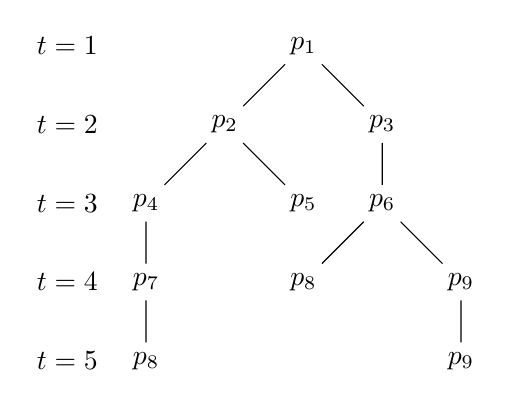
\begin{tikzpicture}
\draw (-3, 0) node {$t=1$};
\draw (-3,-1) node {$t=2$};
\draw (-3,-2) node {$t=3$};
\draw (-3,-3) node {$t=4$};
\draw (-3,-4) node {$t=5$};
\draw (0, 0) node (P1) {$p_1$};
\draw (-1,-1) node (P11) {$p_2$};
\draw (1,-1) node (P12) {$p_3$};
\draw (-2,-2) node (P111){$p_4$};
\draw (0,-2) node (P112) {$p_5$};
\draw (1,-2) node (P121) {$p_6$};
\draw (-2,-3) node (P1111) {$p_7$};
\draw (0,-3) node (P1211) {$p_8$};
\draw (2,-3) node (P1212) {$p_9$};
\draw (-2,-4) node (P11111) {$p_8$};
\draw (2,-4) node (P12121) {$p_9$};

\draw (P1) -> (P11) -> (P111) -> (P1111) -> (P11111);
\draw (P11) -> (P112);
\draw (P1) -> (P12) -> (P121) -> (P1211);
\draw (P121) -> (P1212) -> (P12121);
\end{tikzpicture}
\caption{Transmission Tree}
As we see in the figure above, we can see the effects of a particular perosn 
\end{figure}

For our purposes, a compartmental model is a model of the following form:
\begin{align*}
\vec{x}_i(t+1) = x(t) + \sum_{j \neq i} \alpha_{i,j} \vec{x}_j(t) +  \sum_{j \neq i,k} \alpha_{i,j,k} \vec{x}_j(t) \vec x_k(t)
\end{align*}
%Should I discuss population growth somewhere in this section?
Here $\vec x_i(t)$ is the number of people in compartment $i$ at time $t$, and the above equations model the transition between compartments.  Importantly, $\alpha_{i,j}$ models the rate at which people in compartment $j$ move to compartment $i$, and $\alpha_{i,j,k}$ represents the rate at which an interaction between someone in compartment $j$ and someone in compartment $k$ will cause the person in compartment $j$ to move into compartment $i$.

%Grouped

Individual based models are a larger class of models including the compartmental models we describe here.  In order to model interventions, we will turn our compartmental model described above into an individual based one.  While we started with compartmental models for ease of programming and wide applicability, the methods described here also apply to an arbitrary individual based model. %make sure this is true
In addition to a larger model space, individual based models provide more detail on the transmissions. A compartmental model tells us how many people transition for compartment $i$ to $j$, but an individual based model tells us which people transition.  We will make use of this property to separate the interventions from the underlying process, described below.

We can transform any compartmental model of the form above into an individual based model.  To construct the model, we first consider what would happen if the transitions and interaction terms were independent.  In this case, we can take the intuition behind our compartmental equation and make it explicit.  We let $P_T(p_m = x_j)$ denote the probability that $p_m$ transitions to compartment $x_j$ at time $t$.  We let $P_I(p_m = x_j , p_n)$ be the probability that  at time $t$, $p_m$ is infected by contact with $p_n$.  Then

\begin{align*}
   P_T\left(p_m = x_j \middle| p_m(t) = x_i\right) &= \alpha_{i,j}
\\ P_I\left(p_m = x_j ,p_n \middle| p_m(t) = x_i, p_n(t) = x_k \right) &= \alpha_{i,j,k}.
\end{align*}
However, compartment transitions should be mutually exclusive.  A person can only belong in one compartment at a time.  However, if multiple events occur that change the compartment of $p_m$, we can choose randomly between them, because the compartmental model has an implicit independence assumption within each time step.

We now have a clunkier version of the original model, but one which keeps track of compartment changes \emph{conditional on current compartments}.  This model allows us to compute the compartment change events that occur without knowing who is in which compartment.  This means that if we can generate $P_I(p_m = x_j ,p_n | p_m(t) = x_i, p_n(t) = x_k)$ for all $m$, $n$, $i$, $j$, $k$, and $t$, we would be able to take our initial conditions, come up with some intervention, and run the intervention using those pre generated compartment change events.

We start by assuming that an intervention acts either by \emph{altering transition} probabilities (we will denote this $\beta$), or by \emph{altering compartment} of individuals (we will denote this $\eta$).  We assume that $\beta$ is a function of which people are interacting, their states, the time, and a parameter $\beta^*$ denoting whether the intervention is triggered.  We assume that $\eta$ is a function of the all states of each person up to the current time.  We also assume that both functions have parameters not part of the counterfactual simulation (for example: proportion of people vaccinated).

Unfortunately, at our lab, it is still computationally infeasible to compute all possible transition events on reasonable populations (we used $4$ millionover $365$ days as a benchmark).  However, if we restrict what sorts of interventions we are running, we can instead generate a much smaller set of relevent compartment change events.  In addition to the above constraints, we propose that interventions satisfy the following
\begin{itemize}
\item Interventions do not increase $\alpha$ 
\item Individuals who have their compartment changed by an intervention do not change compartment again.
\item Interventions only affect interactions $\alpha_{i,j,k}$ rather than transitions $\alpha_{i,j}$.
\end{itemize}
While these constraints are relatively limiting, each one can be relaxed/removed at the cost of additional computational resource. %Probably make a supplement about how much resource for which parameters?

While we make strong assumptions, there are still a number of intervention startegies that meet them.  Interventions that reduce infectious interactions like hygiene interventions, social distnacing, and vaccines that aren't fully innoculating all satisfy the assumptions.  As do interventions which remove part of the population entirely, like school closings, and quarantine.  Even vaccination and treatment interventions satisfy these assumptions in the case that they grant lifelong immunity.

\subsection*{Example: Influenza}

\begin{figure}
\label{fig:sir}
\begin{center}
\begin{tikzpicture}
\draw (0,0) node (S) {$S$};
\draw (2,0) node (I) {$I$};
\draw (4,0) node (R) {$R$};
\draw[->] (S) -- node [pos = .5, label=$\frac{\beta}{N} I$]{} (I);
\draw[->] (I) -- node [pos = .5, label=$\gamma$]{} (R);
\end{tikzpicture}
\end{center}
\caption{Influenza Compartmental Model}
\end{figure}

%We will now show a specific example of the above process applied to Influenza and several interventions.  For a single season, Influenza can be modeled using an SIR model\cite{}, as in Figure \ref{fig:sir}.  Following the example of %FIX ME
, we use $\alpha_{I,S,I} = \frac{\beta}{N} = ??$ %FIX ME
, and $\alpha_{R,I} = \gamma = ??$ %FIX ME
.  We can turn this into transition probabilities and obtain
\begin{align*}
   P_T\left(p_m = R \middle| p_m(t) = I\right) &= ?? %FIX ME
\\ P_I\left(p_m = I ,p_n \middle| p_m(t) = S, p_n(t) = I \right) &= ??%FIX ME
\end{align*}
These probabilities are already mutually exclusive, so we don't have to worry about multiple simultaneous transitions.  We will look at several possible interventions against influenza.

\paragraph{None}
In order to have something to compare our interventions to, we consider the effect of no intervention at all.  For $\beta$, we always return $1$ in order to never change any case.  For $\eta$, we never make any changes.
\paragraph{Vaccination}
The first real intervention we will examine is a vaccination campaign.  At some time $t^*$, a group comes in and randomly vaccinates some proportion $p_{\text{vac}}$ of susceptibles..  For $\beta$, we always return $1$.  However for $\eta$, we don't make any changes, unless $t$ is $t^*$, and then we move $p_{\text{vac}}$ of the people in compartment $S$ to compartment $R$.
\paragraph{Treatment}
Another way we might intervene is by speeding the recovery of individuals.  The ????????? %FIX ME  There's some medicine thing that goes here cytovax or something? idr
causes individuals to stop being infectious.  Then our $\beta$ is still always $1$, but for $\eta$, we move some proportion of the populaion of compartment $I$ to compartment $R$ at each time step.
In other words, we never remove an existing infection, and we never chnage the state of anyone.
\paragraph{Social Distancing}
As the flu becomes more common, people become more aware of their social contacts, and are more likely to avoid contacts who might have the flu \cite{}.  For simplicity, we say that if the number of cases rises above a threshold $I^*$, people become less likely to have potentially infectious contact by a factor of $\sigma$.  So then $\beta$ is $1$ when $\beta^* = 0$, and $\sigma$ when $\beta^* = 1$.  $\beta^* = 1$ if $\| I \| >= I^*$, and $\beta^* = 0$ otherwise.
\section{Results}
\section{Discussion}

\bibliography{bib}{}
\bibliographystyle{plain}
\end{document}